\chapter{Evaluation}

\begin{figure*}
    \centering
    \small
     \begin{tabular}{l|c|r|l}
       \bf Application        & \bf Type    & \bf LoC & \bf Policies   \\
      \hline
       Atomic~\cite{atomic} (v0.34.2)       & Graph DB    & 9.6k   & Access Control                                 \\
       Contile~\cite{contile} (v1.11.0)     & Advertising & 4.9k     & Purpose Limitation                           \\
       Freedit~\cite{freedit} (v0.6.0-rc.3) & Social      & 6.6k     & Data Retention/Expiration                     \\
       Hyperswitch~\cite{hyperswitch} (v0.2.0)   & Payments    & 198.9k     & Credential Security, Limited Data Collection  \\
       Lemmy~\cite{lemmy} (v0.16.6)        & Social      & 31.4k   & Access Control                               \\
       Plume~\cite{plume} (v0.7.2)         & Blogging    & 21.4k   & Data Deletion                                \\
       WebSubmit~\cite{websubmit} (v1.0)       & Homework    & 1.6k    & Data Deletion, Access Control     \\
    \end{tabular}
    \caption{Case study applications with code size and policies.}
    \label{f:apps}
   \end{figure*}

We evaluate \syslang{} against seven third-party Rust applications to answer four questions:
%
\begin{enumerate}[nosep]
    \item Can \syslang's grammar express real-world \policies? (\S\ref{sec:expressivity})
    \item How do \syslang's abstractions impact policy precision and correctness?(\S\ref{sec:precision})
    \item Are \syslang's policies efficient enough for practical use? (\S\ref{sec:efficiency})
    \item What is the effort required to encode policies in \syslang? (\S\ref{sec:accessibility})
\end{enumerate}
%

We tried to pick popular applications spanning different policy domains.
%
We summarize the applications in~\Cref{f:apps}.

\section{Expressivity}
\label{sec:expressivity}
%
We found that \syslang{} could express all of the policies that we defined for these applications.
%
In cases where the policy was inherently dynamic, we defined static approximations.
%
For example, a GDPR data deletion policy would state that some \controller{} deletes \emph{all} of a user's data.
%
\sys{} cannot verify that the application actually deletes all of the user's data,
since the exact contents of that data are only known at runtime.
%
However, it can ensure that for each type marked \lstinline[language=CNL]|@@user_data@@|, 
there is some data of that type that goes to a \lstinline[language=CNL]|"deleter"|.
%
This policy is expressive enough to find bugs where applications forget to delete a given type of user data,
but cannot catch bugs where an application only deletes \emph{some} of the data of a given type.
%

While we were able to express all of the policies for these applications,
we do not expect that \syslang{} could express every privacy policy.
%
For example, our \syslang{} prototype cannot express policies that rely on direct dependencies 
or more than five levels of nested expressions~(\Cref{sec:direct-limits,sec:other-limits}).
%
It also cannot express policies that require more fine-grained reasoning about particular source code
entities, like arguments.
%
As an example, we present a (simplified) version of one of our policies for WebSubmit, a homework submission system.
%
WebSubmit sends students feedback through email using the function |send_email(recipient, sender, content)|.
%
A \ce{} may want to enforce that if \lstinline[language=CNL]|@@sensitive@@| data is sent,
the recipient is an administrator.
%
However, if the \ce{} simply checked that data marked \lstinline[language=CNL]|@@admin@@| goes to \emph{some} |recipient|,
then code like this would pass the policy:
\begin{lstlisting}[language=Rust]
    send_email(admin@cs.brown.edu, student1@cs.brown.edu, benign_data);
    send_email(student1@cs.brown.edu, student2@cs.brown.edu, sensitive_data);
\end{lstlisting}
The second |send_email| call is unsafe because sensitive data is sent to a student, not an administrator.
%
However, because the first, unrelated |send_email| recipient is an administrator, 
\sys{} would see that some recipient is an administrator and the policy would pass.
%
To prevent this bug, a \ce{} could make their policy more precise: if data marked \lstinline[language=CNL]|@@sensitive@@| goes to |content|,
then data marked \lstinline[language=CNL]|@@admin@@| goes to |recipient| \emph{in the same} |send_email| \emph{operation}.
%
\syslang{} cannot express this policy exactly.
%
It can get close--it can express that data marked \lstinline[language=CNL]|@@admin@@| goes to the same operation,
but it cannot enforce that it goes to the |recipient| argument specifically.
%
Thus, the \syslang{} version of the policy would allow this (buggy) code to pass:
\begin{lstlisting}[language=Rust]
    send_email(student1@cs.brown.edu, student2@cs.brown.edu, 
                "admin@cs.brown.edu's credit card number is [...]");
\end{lstlisting}
%
This code is incompliant because it sends sensitive data to a student,
but \syslang{}'s policy would not catch it because \lstinline[language=CNL]|@@admin@@| goes to 
the operation through the |content| argument.
%
\sys{}'s Graph Query API can enforce that the administrator goes to the |recipient| argument,
so it is possible to write a native Rust policy that catches this bug.

\section{Precision}
\label{sec:precision}
\syslang{} policies do not support the same degree of precision as native Rust polices~(\Cref{sec:interface,sec:direct-limits}).
%
We evaluate to what extent this loss of precision affects the accuracy of \syslang{} policies.

For each application, we wrote Graph Query API policies and equivalent \syslang{} policies.
%
The Graph Query API policies leveraged functionality that is out of scope for \syslang{}
(e.g., reasoning about the direct siblings of a marked node).
%
We ran these policies on compliant and incompliant versions of the applications.
%
We found that both sets of policies were correct for every application,
i.e., passed for the compliant versions and failed for the incompliant ones.
%
This result is a promising indicator that \syslang's worse precision is acceptable in practice.

\section{Efficiency}
\label{sec:efficiency}
For each application, we compare the total execution time of its Graph Query API policies
and their \syslang{} policies.
%
To avoid the variance of a single run unduly affecting the result, we average the results over 10 runs each.
%
We would expect \syslang{} policies to be slower on average because of its compiler limitations (\S\ref{sec:code-limits}).

~\Cref{f:times,f:percentages} compare the \syslang{} and Graph Query API policy execution times.
%
We found that \syslang{} policies are 2-12\% slower than their Graph Query API counterparts.
%
The one exception is WebSubmit, which was 0.5\% faster than the Rust API policies.
%
However, the WebSubmit policies run quickly (~30ms),
so in any given run, a difference of a few milliseconds causes this percentage to vary widely.

These results demonstrate that \syslang{} policies incur an acceptable overhead compared to native Rust policies.

\begin{figure}
    \begin{centering}
        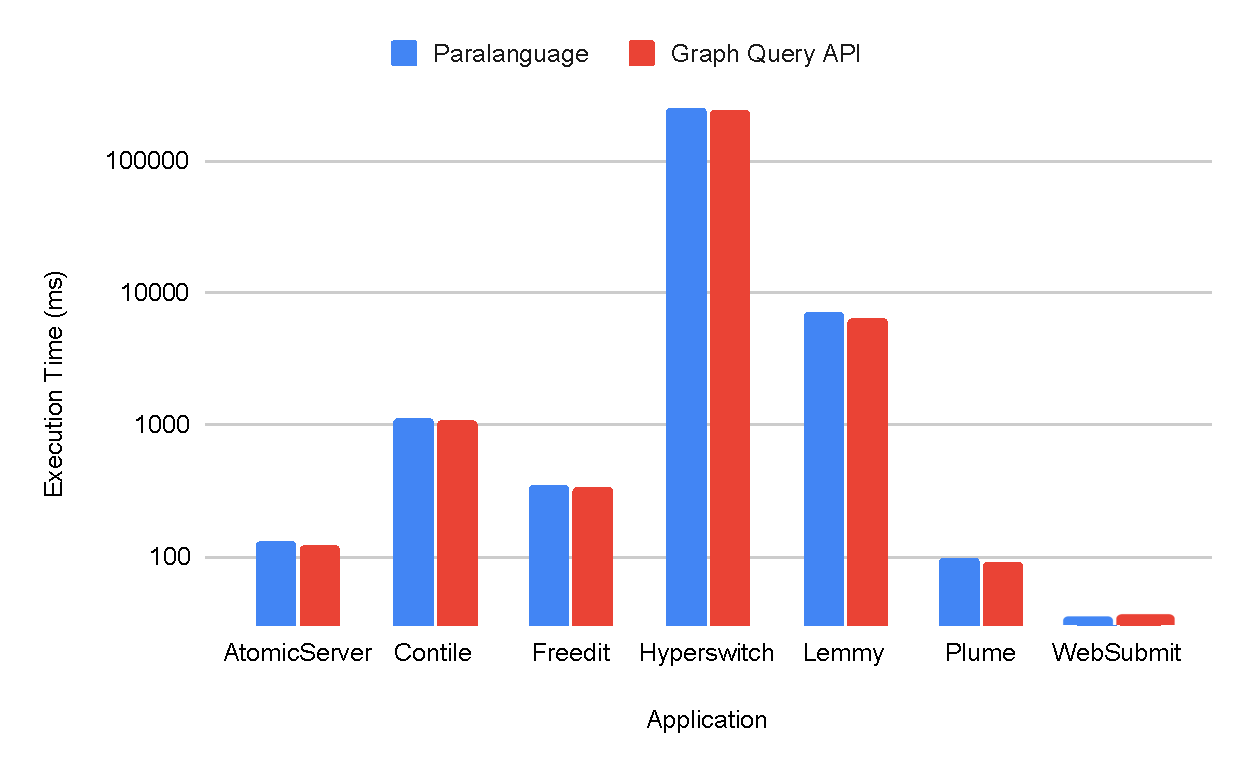
\includegraphics[scale=0.6]{graphics/times.pdf}
        \caption{\syslang{} and Graph Query policy execution times, averaged across 10 runs.}
        \label{f:times}
    \end{centering}
\end{figure}
%
\begin{figure}
    \begin{tabular}{|l|p{3cm}|p{3.5cm}|p{2cm}|p{3cm}|}
        \hline
        \textbf{Application} & \textbf{\syslang{} Time (ms)} & \textbf{Graph Query API Time (ms)} & \textbf{Difference (ms)} & \textbf{\syslang{} \% Slower} \\ \hline
        AtomicServer & 127.92    & 118.8     & 9.12    & 7.68  \\ \hline
        Contile      & 1109.14   & 1064.43   & 44.71   & 4.2   \\ \hline
        Freedit      & 347.57    & 339.85    & 7.72    & 2.27  \\ \hline
        Hyperswitch  & 251044.37 & 241890.42 & 9153.95 & 3.78  \\ \hline
        Lemmy        & 7026.23   & 6277.3    & 748.93  & 11.93 \\ \hline
        Plume        & 95.63     & 88.86     & 6.77    & 7.62  \\ \hline
        WebSubmit    & 29.89     & 30.07     & -0.18   & -0.6  \\ \hline               
        \end{tabular}
        \caption{Comparison of \syslang{} and Graph Query API policy execution times.}
        \label{f:percentages}
\end{figure}

\section{Effort}
\label{sec:accessibility}

We evaluate the effort required to encode policies in \syslang{}.
%
Ideally, we would have conducted a user study with users unfamiliar with the system.
%
However, due to time limitations, we instead summarize our experience (as the authors of \syslang{}) writing policies.
%

\paragraph{Policy Strictness:} We find that the effort required to encode policies in \syslang{} is proportional to the strictness of the policy.
%
For example, take the AtomicServer application, a graph-based database.
%
% To update a database resource, users commit a record of their changes.
% %
% % Before applying the commit, the application must verify that the user is permitted to modify the resource.
% %
A previous version of the application failed to verify that the 
user was permitted to modify a database resource before applying the change.
%
% A (simplified) version of the fixed source code is below.
% %
% \begin{lstlisting}[language=Rust]
%     impl Commit {
%         pub fn update_resource(&self, store: &Database) -> AtomicResult<Resource> {
%             let commit_resource: Resource = self.clone().into_resource(store)?;
%             /* fix -- move check_required_props above add_resource */
%             resource.check_required_props(store)?; 
%             store.add_resource(&commit_resource)?;
%         }
%     }
% \end{lstlisting}
%
% Our Graph Query API policy writers had markers for both the |Commit| and |Resource| types.
% %
% Their policy enforced that if a |Commit| is stored,
% the user was authorized under the permissions of the |Resource|.
% %
% They derived this policy by reasoning backward from the source code--the \dev{} comments, e.g. the ``Save the Commit to the Store'' comment,
% reason about storing the commit.
% %
% When I was writing the \syslang{} policy, however, I was not thinking about the source code implementation of |Commit|s.
% %
% Instead, I reasoned that if the database resource was what was modified,
% then there is no reason to care about the particular commit record of the changes that get stored alongside that resource.
%
We encode this policy in \syslang{} by checking that if a \lstinline[language=CNL]|"database resource" goes to "update"|,
\lstinline[language=CNL]|"database resource" goes to "auth check"| and 
\lstinline[language=CNL]|"auth check" affects whether "update" happens|.
%
This policy fails on the buggy version of the application and passes on the fixed version.

Prior to this work, we wrote a version of this policy in the Graph Query API.
%
This policy was stricter: it also included the implementation-specific notion of \emph{commits}.
%
Commits are records of modifications to a resource (analogous to Git commits).
%
Our Graph Query API policy enforced that a commit had transitive data influence on the modified resource.
%
This assertion is not necessary to catch this particular permission check bug, 
but it would catch a bug where the application updated the wrong resource (i.e., one unaffiliated with a commit).

To write this stricter policy in \syslang{}, \ces{} and \devs{} must expend more effort.
%
The \ce{} would need more advanced implementation knowledge: 
they would need to understand the notion of commits and how they interact with resources.
%
They may need to consult with the \dev{} to update the policy,
and the \dev{} would need to apply (and maintain) more markers.

By abstracting away details of the source code,
\syslang{} encourages the \ce{} to think about the minimum set of concepts
necessary to express their policy.
%
While this approach can simplify policies,
it may cause the \ce{} to miss opportunities to strengthen their policies with implementation-specific assertions.
%
% Graph Query API policies are less likely to suffer this problem because they require
% more advanced knowledge of programming and the application's PDG,
% which makes it more likely that they are written by an \dev{}
% familiar with the implementation.
%
% In these cases, we count on the developer to assess the policy they receive from the \ce{}
% and make suggestions for improvements as they see fit.
% %
To write stricter policies in \syslang, the \ce{} likely needs to consult with the developer.

\paragraph{Bullets:} We found that for some of the policies, 
our first attempt to express them required more levels of bullets than \sys{} supports~(\Cref{sec:other-limits}).
%
We refactored the policies to use definitions, 
which allowed us to express the policies with fewer nested expressions.
%
We found that this process made our final policies easier to read,
even if it took us longer to write them.